% =============================================================================
%  PDC Assignment 3 - slides: EXACTLY 6 slides (1 intro + 5 case studies)
%  Build:  cd slides && make      -> GroupXX_slides.pdf
%  Member B: fill in the CS3 and CS4 frames (marked TODO).
% =============================================================================
\documentclass[aspectratio=169,10pt]{beamer}
\usetheme{default}
\usecolortheme{default}
\setbeamertemplate{navigation symbols}{}
\setbeamertemplate{footline}[frame number]
\setbeamerfont{frametitle}{size=\large,series=\bfseries}
\usepackage{tikz}
\usepackage{booktabs}
\graphicspath{{../report/figures/}}

\newcommand{\groupno}{XX}
\newcommand{\memberA}{Eshaal Rehamtullah}
\newcommand{\memberB}{Atika Hussain}
\newcommand{\todo}[1]{\textcolor{red}{\textbf{[TODO: #1]}}}
\newcommand{\insight}[1]{\begin{block}{Key insight}#1\end{block}}
\newcommand{\trynext}[1]{\textbf{Next:} #1}

\begin{document}

% ---------------------------------------------------------------- 1. intro
\begin{frame}{PDC Assignment 3 --- Five Parallel Case Studies}
\begin{columns}[T]
\column{0.48\textwidth}
\textbf{Team}
\begin{itemize}\small
  \item \memberA\ (23L-0648) --- CS1 heat (MPI), CS2 $k$-mers (OpenMP), CS5 sample sort (MPI)
  \item \memberB\ (23L-0570) --- CS3 Monte Carlo, CS4 PageRank (OpenMP)
\end{itemize}
\textbf{Machine}
\begin{itemize}\small
  \item AMD Ryzen 9 7940HS: 8 cores / 16 threads, 16\,MB L3, 7.4\,GB RAM
  \item Ubuntu 24.04 (WSL2), gcc 13.3 \texttt{-O3}, Open MPI 4.1.6
  \item Every time = median of 3 runs, $p \le 8$
\end{itemize}
\column{0.5\textwidth}
\textbf{Model per case study}\\[0.3em]
\small
\begin{tabular}{@{}lll@{}}
\toprule
CS1 & Heat diffusion   & MPI, 2-D halo exchange \\
CS2 & $k$-mer counting & OpenMP, private histograms \\
CS3 & Monte Carlo      & OpenMP, per-thread RNG streams \\
CS4 & PageRank         & OpenMP, pull vs push \\
CS5 & Sample sort      & MPI, Alltoallv \\
\bottomrule
\end{tabular}
\end{columns}
\end{frame}

% ---------------------------------------------------------------- 2. CS1
\begin{frame}{CS1 Heat diffusion --- MPI}
\begin{columns}[T]
\column{0.42\textwidth}
\small
\textbf{Problem:} update an $N{\times}N$ plate for 500 steps; each cell mixes with its 4 neighbours.\\[0.4em]
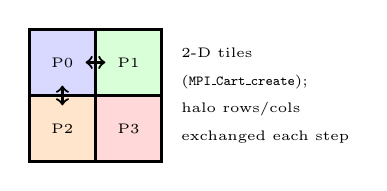
\begin{tikzpicture}[scale=0.42]
  \fill[blue!15] (0,2) rectangle (2,4); \fill[green!15] (2,2) rectangle (4,4);
  \fill[orange!20] (0,0) rectangle (2,2); \fill[red!15] (2,0) rectangle (4,2);
  \draw[very thick] (0,0) rectangle (4,4); \draw[very thick] (0,2)--(4,2); \draw[very thick] (2,0)--(2,4);
  \node at (1,3) {\tiny P0}; \node at (3,3) {\tiny P1}; \node at (1,1) {\tiny P2}; \node at (3,1) {\tiny P3};
  \draw[<->,thick] (1.7,3)--(2.3,3); \draw[<->,thick] (1,1.7)--(1,2.3);
  \node[right,align=left] at (4.3,2) {\tiny 2-D tiles\\[-2pt]\tiny (\texttt{MPI\_Cart\_create});\\[-2pt]\tiny halo rows/cols\\[-2pt]\tiny exchanged each step};
\end{tikzpicture}
\insight{Small grid ($N{=}1024$, fits in cache): \textbf{4.7$\times$} on 8 cores.
Big grid ($N{=}4096$, 268\,MB): only \textbf{1.6$\times$}, with comm.\ just 6\% of the
time $\Rightarrow$ the shared \textbf{memory bus} is the limit, not MPI.}
\trynext{cache blocking / several steps per halo exchange (wider halo).}
\column{0.56\textwidth}
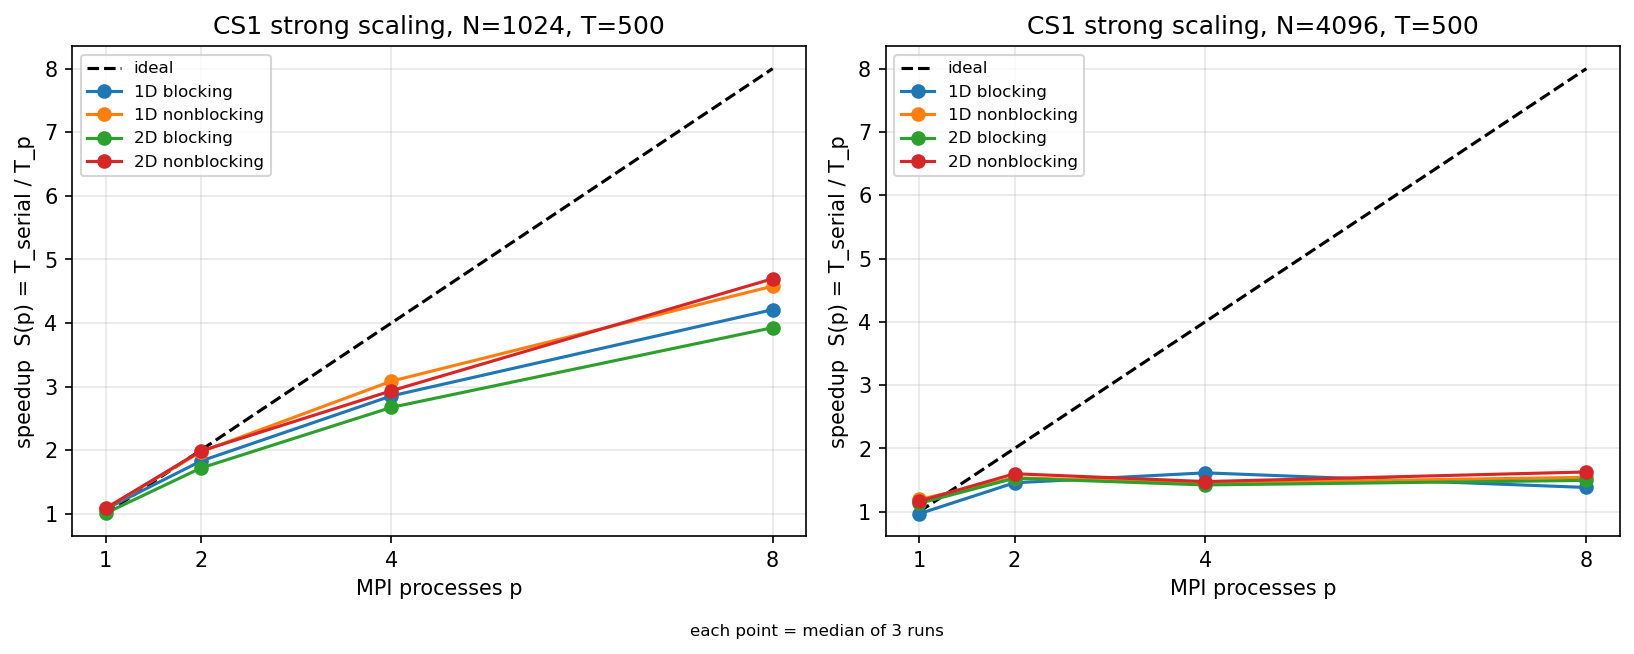
\includegraphics[width=\textwidth]{cs1_strong_scaling.png}\\[-0.3em]
{\tiny Non-blocking overlap hid $\approx$43\% of comm.\ time ($N{=}1024$, $p{=}8$). Median of 3 runs.}
\end{columns}
\end{frame}

% ---------------------------------------------------------------- 3. CS2
\begin{frame}{CS2 $k$-mer counting --- OpenMP}
\begin{columns}[T]
\column{0.42\textwidth}
\small
\textbf{Problem:} count every length-$k$ substring of a $10^8$-base DNA string (histogram with $4^k$ bins).\\[0.4em]
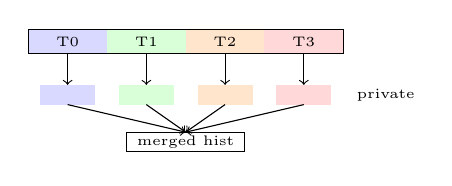
\begin{tikzpicture}[scale=0.5]
  \foreach \i/\c in {0/blue!15,1/green!15,2/orange!20,3/red!15}
   { \fill[\c] ({2*\i},0) rectangle ({2*\i+2},0.6); \node at ({2*\i+1},0.3) {\tiny T\i};
     \fill[\c] ({2*\i+0.3},-1.3) rectangle ({2*\i+1.7},-0.8); \draw[->] ({2*\i+1},0)--({2*\i+1},-0.8);
     \draw[->] ({2*\i+1},-1.3)--(4,-2.0); }
  \draw (0,0) rectangle (8,0.6);
  \draw (2.5,-2.5) rectangle (5.5,-2.0); \node at (4,-2.25) {\tiny merged hist};
  \node[right] at (8.1,-1.05) {\tiny private};
\end{tikzpicture}
\insight{Race (A) lost \textbf{102{,}012} counts. Private copies win for $k{=}8$
(\textbf{5.0$\times$}, 2\,MB extra) but lose to atomics for $k{=}12$ (512\,MB extra,
everything misses cache). False sharing: \textbf{5.1$\times$ slower} without padding.}
\trynext{share one histogram per core pair / sort-based counting for $k{=}12$.}
\column{0.56\textwidth}
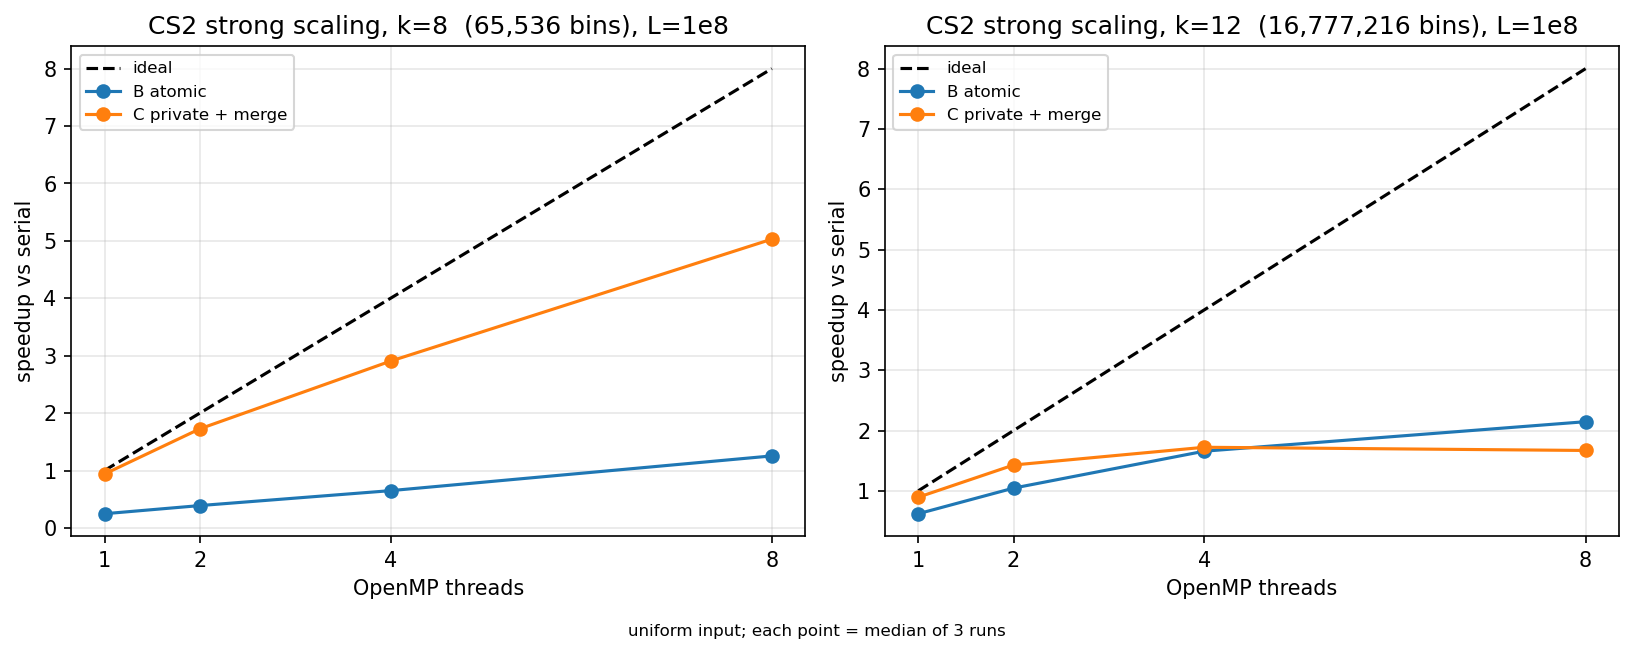
\includegraphics[width=\textwidth]{cs2_strong_scaling.png}\\[-0.3em]
{\tiny B = \texttt{omp atomic}, C = private histograms + merge. Median of 3 runs.}
\end{columns}
\end{frame}

% ---------------------------------------------------------------- 4. CS3
\begin{frame}{CS3 Monte Carlo option pricing --- OpenMP}
\begin{columns}[T]
\column{0.42\textwidth}
\small
\textbf{Problem:} price a European call ($S_0{=}K{=}100$, $r{=}0.05$, $\sigma{=}0.2$, $T{=}1$) via $M$ GBM paths (Box--Muller) vs.\ Black--Scholes (\texttt{10.4506}).\\[0.4em]
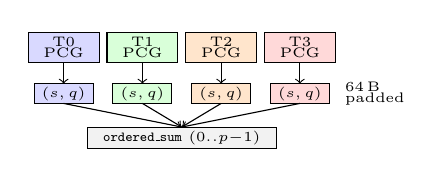
\begin{tikzpicture}[scale=0.5, every node/.style={font=\tiny}]
  \foreach \i/\c in {0/blue!15,1/green!15,2/orange!20,3/red!15}
   { \fill[\c] ({2*\i},0) rectangle ({2*\i+1.8},0.75);
     \draw ({2*\i},0) rectangle ({2*\i+1.8},0.75);
     \node[align=center] at ({2*\i+0.9},0.38) {T\i\\[-2pt]PCG};
     \draw[->] ({2*\i+0.9},0)--({2*\i+0.9},-0.55);
     \fill[\c] ({2*\i+0.15},-1.05) rectangle ({2*\i+1.65},-0.55);
     \draw ({2*\i+0.15},-1.05) rectangle ({2*\i+1.65},-0.55);
     \node at ({2*\i+0.9},-0.8) {$(s,q)$};
     \draw[->] ({2*\i+0.9},-1.05)--(3.9,-1.65); }
  \node[right,align=left] at (7.8,-0.8) {64\,B\\[-2pt]padded};
  \draw[fill=gray!10] (1.5,-2.2) rectangle (6.3,-1.65);
  \node at (3.9,-1.92) {\texttt{ordered\_sum} ($0..p{-}1$)};
\end{tikzpicture}
\insight{At $M{=}2\text{M}, p{=}4$: \texttt{perthread} hits \textbf{49.01\,Mpaths/s} (0.0408\,s); a \texttt{shared} locked RNG is \textbf{6.4$\times$ slower} (0.2601\,s, non-reproducible); \texttt{sameseed} correlates streams. \texttt{blocks} ($B{=}4096$) is \textbf{bit-identical} across $p{=}1,3,7$.}
\trynext{full $M{\ge}10^8$ scaling sweep ($p{=}1..8$) + antithetic variates / SIMD Box--Muller.}
\column{0.56\textwidth}
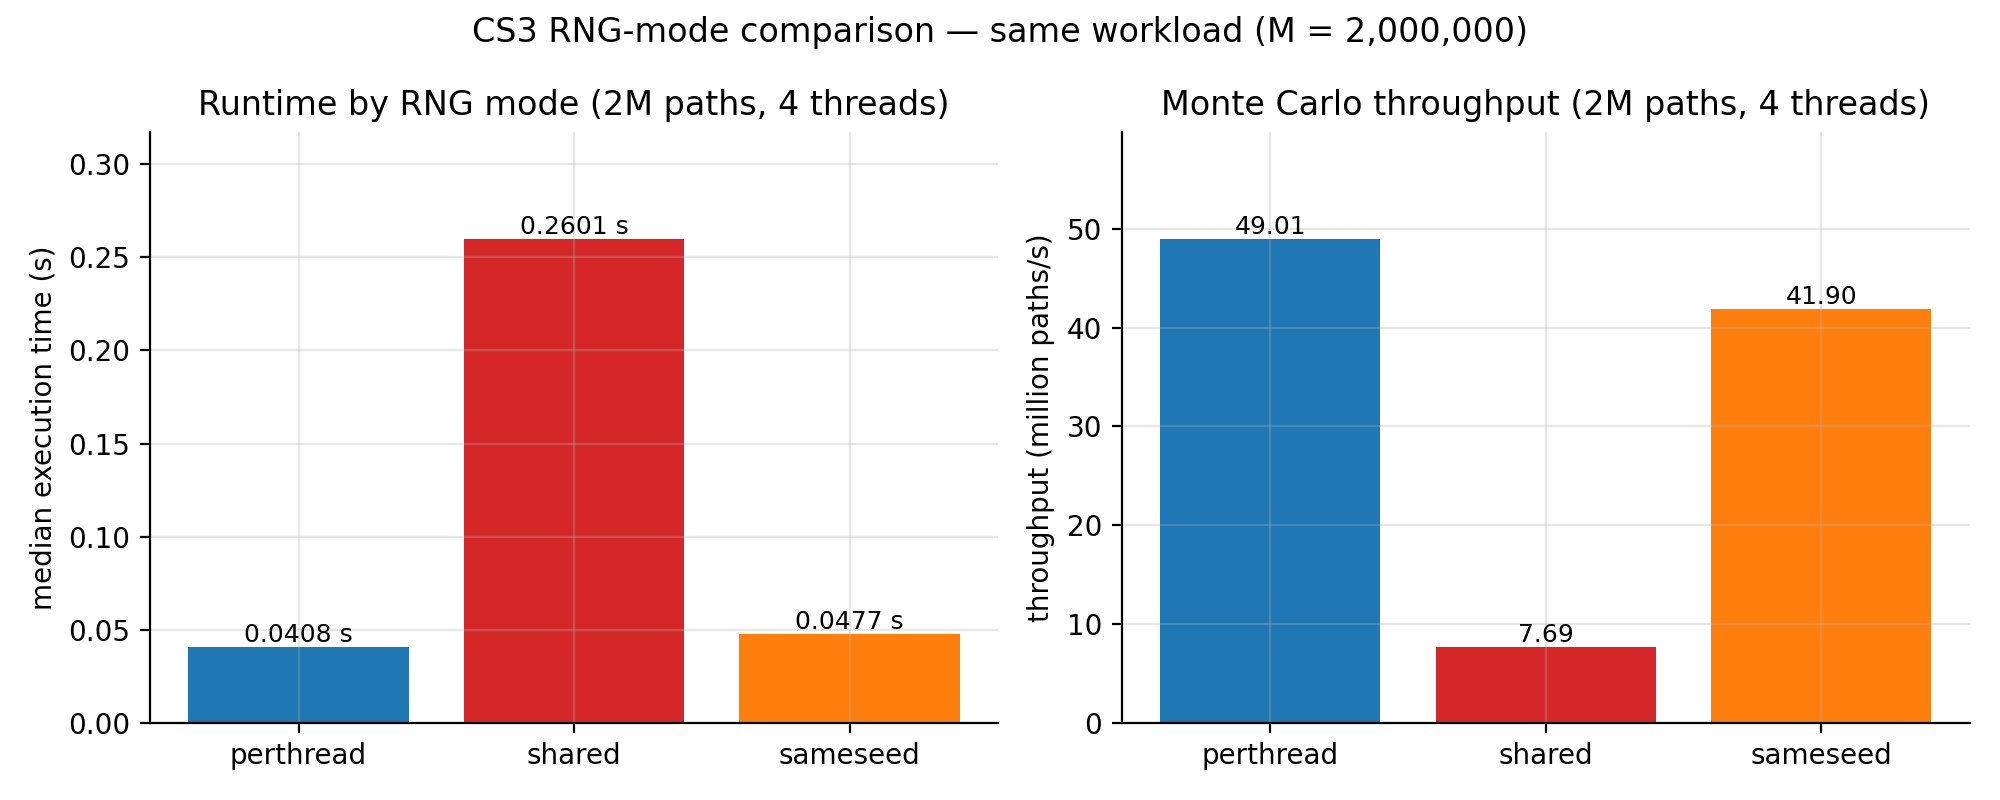
\includegraphics[width=\textwidth]{cs3_rng_performance.png}\\[-0.3em]
{\tiny RNG modes at $M{=}2\text{M}, p{=}4$ (median of 3 runs). At $M{=}4\text{M}, p{=}4$: \texttt{perthread} $= 10.4362 \pm 0.0074$ SE (BS $= 10.4506$); \texttt{parallel -t 1} matches \texttt{serial} bit-for-bit (\texttt{0x1.4e26e7b5ac647p+3}).}
\end{columns}
\end{frame}

% ---------------------------------------------------------------- 5. CS4
\begin{frame}{CS4 PageRank --- OpenMP}
\begin{columns}[T]
\column{0.42\textwidth}
\small
\textbf{Problem:} iterate PageRank ($d{=}0.85$, $\varepsilon{=}10^{-9}$, 24 iters) on R-MAT scale-20 CSR ($n{=}1.05\text{M}$, $m{=}16.08\text{M}$ edges).\\[0.4em]
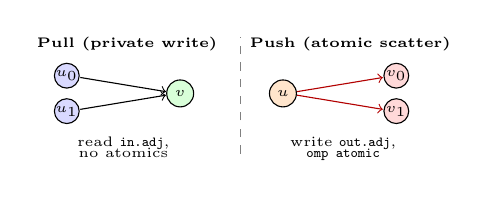
\begin{tikzpicture}[scale=0.45, every node/.style={font=\tiny}]
  \node[font=\tiny\bfseries] at (1.9,2.1) {Pull (private write)};
  \draw[fill=blue!15] (0.2,1.2) circle (0.35) node {$u_0$};
  \draw[fill=blue!15] (0.2,0.2) circle (0.35) node {$u_1$};
  \draw[fill=green!15] (3.4,0.7) circle (0.38) node {$v$};
  \draw[->] (0.58,1.15)--(3.0,0.75);
  \draw[->] (0.58,0.25)--(3.0,0.65);
  \node[below,align=center] at (1.8,-0.25) {read \texttt{in.adj},\\[-2pt]no atomics};
  \draw[dashed,gray] (5.1,-1.0)--(5.1,2.3);
  \node[font=\tiny\bfseries] at (8.2,2.1) {Push (atomic scatter)};
  \draw[fill=orange!20] (6.3,0.7) circle (0.38) node {$u$};
  \draw[fill=red!15] (9.5,1.2) circle (0.35) node {$v_0$};
  \draw[fill=red!15] (9.5,0.2) circle (0.35) node {$v_1$};
  \draw[->,red!70!black] (6.7,0.75)--(9.12,1.15);
  \draw[->,red!70!black] (6.7,0.65)--(9.12,0.25);
  \node[below,align=center] at (8.0,-0.25) {write \texttt{out.adj},\\[-2pt]\texttt{omp atomic}};
\end{tikzpicture}
\insight{\texttt{pull} static stalls at \textbf{1.83$\times$} ($p{=}8$, imbalance $R{=}2.18$); \texttt{dynamic,256} hits \textbf{4.08$\times$} (0.348\,s, 1110\,M\,edges/s). \texttt{push} with atomics is \textbf{4.1$\times$ slower} than \texttt{pull} at $p{=}4$ (atomics add \textbf{+122\%} at $p{=}1$ plus hub contention).}
\trynext{degree-ordered / cache-blocked CSR for \texttt{contrib[]} locality, or hybrid push--pull.}
\column{0.56\textwidth}
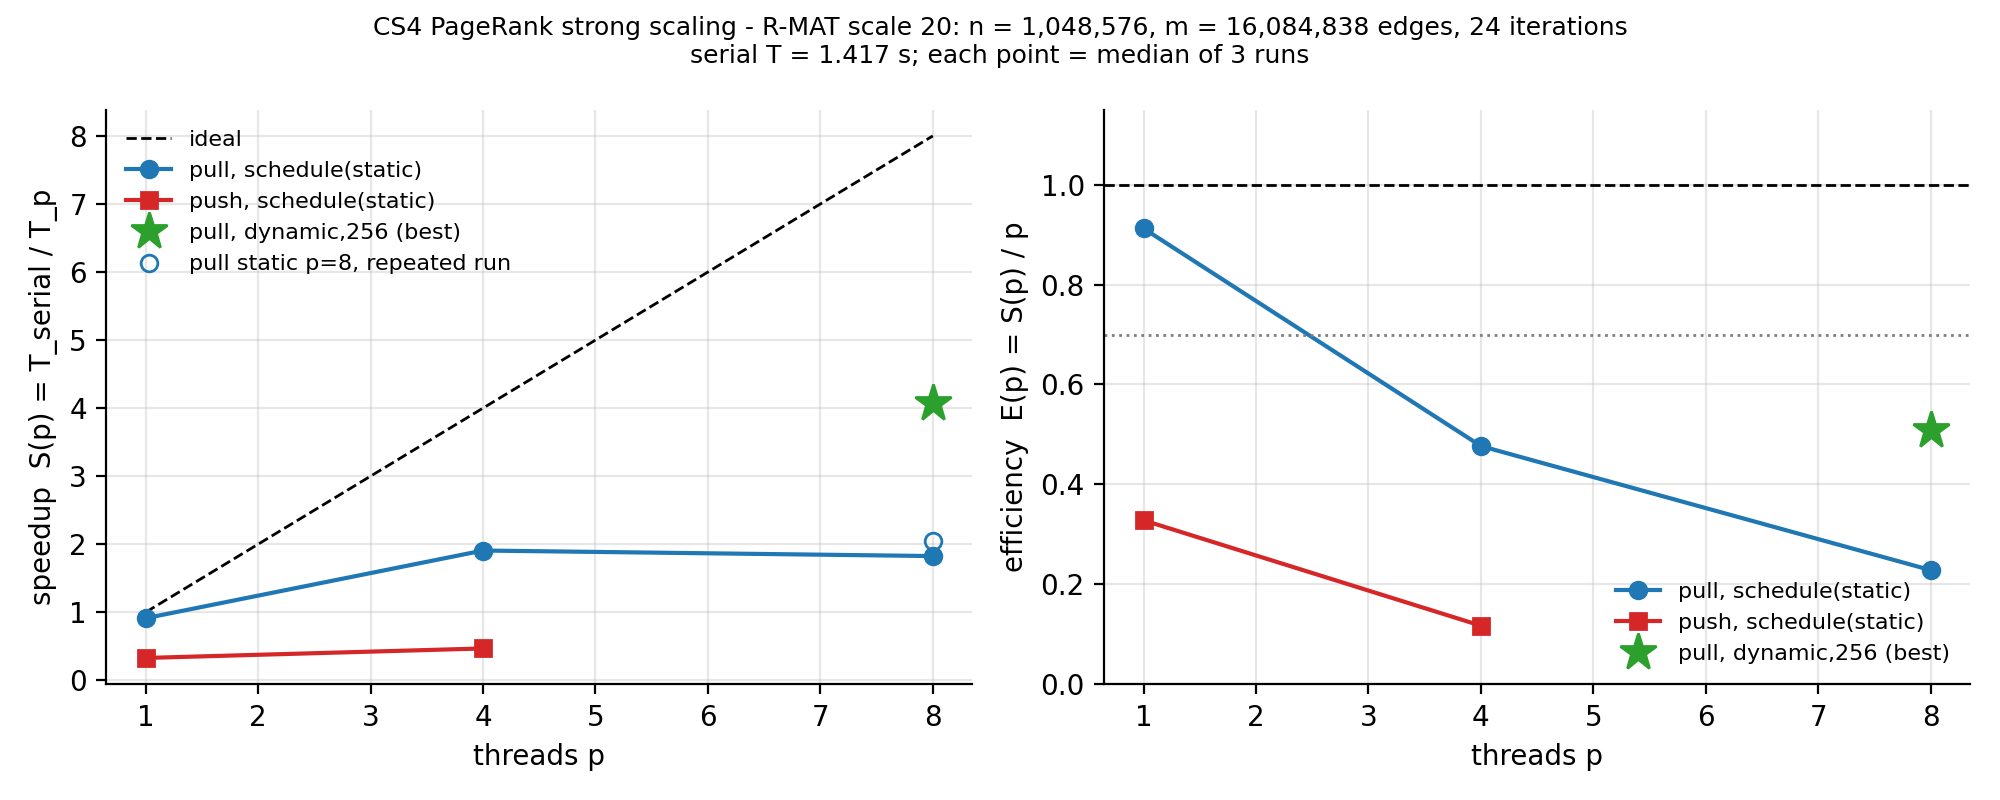
\includegraphics[width=\textwidth]{cs4_strong_scaling.png}\\[-0.3em]
{\tiny Serial $T{=}1.4175$\,s; median of 3 runs. At $p{=}8$ (\texttt{pull}): \texttt{dynamic,256} $= 0.348$\,s (4.08$\times$), edge-balanced $= 0.551$\,s (2.57$\times$), \texttt{static} $= 0.776$\,s (1.83$\times$), \texttt{guided,64} $= 0.878$\,s (1.61$\times$).}
\end{columns}
\end{frame}

% ---------------------------------------------------------------- 6. CS5
\begin{frame}{CS5 Distributed sample sort --- MPI}
\begin{columns}[T]
\column{0.42\textwidth}
\small
\textbf{Problem:} globally sort $10^8$ 32-bit keys spread over $p$ processes.\\[0.4em]
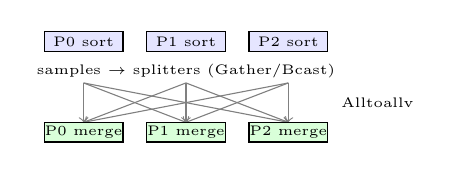
\begin{tikzpicture}[scale=0.5, every node/.style={font=\tiny}]
  \foreach \i in {0,1,2} { \draw[fill=blue!10] ({2.6*\i},0) rectangle ({2.6*\i+2},0.5); \node at ({2.6*\i+1},0.25) {P\i\ sort}; }
  \node at (3.6,-0.5) {samples $\rightarrow$ splitters (Gather/Bcast)};
  \foreach \i in {0,1,2} \foreach \j in {0,1,2} \draw[->,gray] ({2.6*\i+1},-0.8) -- ({2.6*\j+1},-1.8);
  \node[right] at (7.3,-1.3) {Alltoallv};
  \foreach \i in {0,1,2} { \draw[fill=green!15] ({2.6*\i},-2.3) rectangle ({2.6*\i+2},-1.8); \node at ({2.6*\i+1},-2.05) {P\i\ merge}; }
\end{tikzpicture}
\insight{\textbf{7.3$\times$} on 8 cores (uniform). Local sort is 87\% of the time;
Alltoallv is only 0.07\,s. With only 16 distinct values one rank gets
\textbf{1.5$\times$} the average, since equal keys cannot be split.}
\trynext{break ties with (key, position) so duplicates can be split.}
\column{0.56\textwidth}
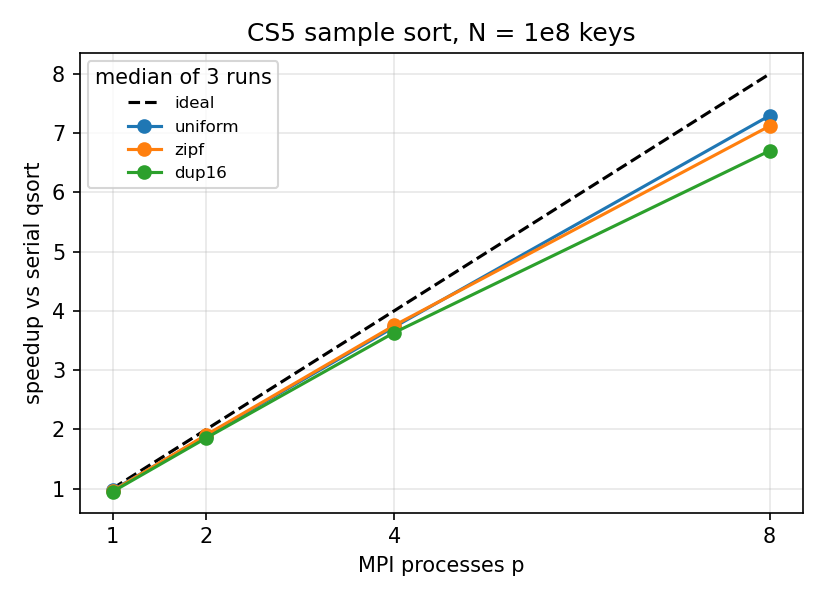
\includegraphics[width=0.49\textwidth]{cs5_strong_scaling.png}\hfill
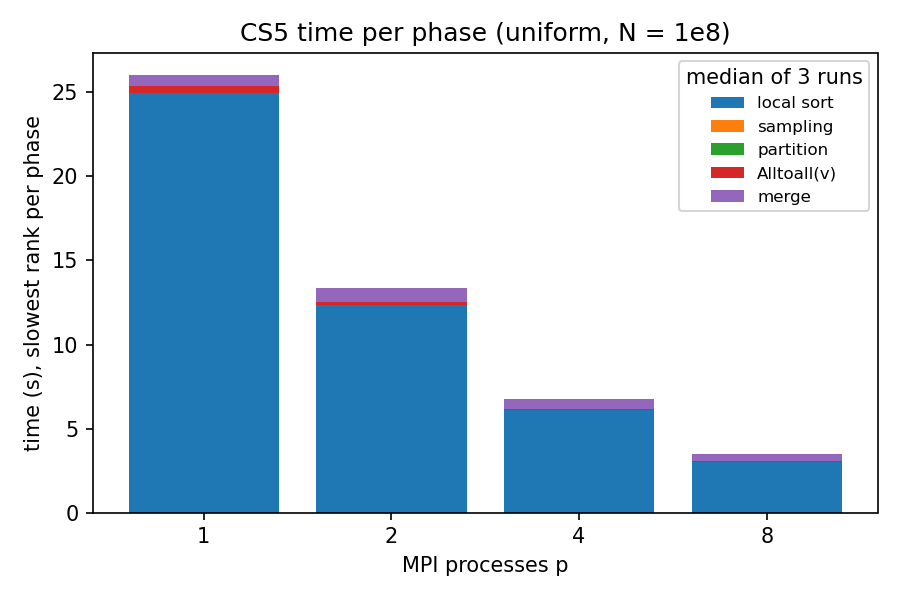
\includegraphics[width=0.49\textwidth]{cs5_phase_breakdown.png}\\[-0.3em]
{\tiny Left: speedup vs.\ serial qsort ($N{=}10^8$). Right: time per phase (slowest rank), uniform. Median of 3 runs.}
\end{columns}
\end{frame}

\end{document}
